\documentclass[11pt]{article}
\usepackage[T1]{fontenc}
\usepackage[utf8]{inputenc}
\usepackage{lmodern}
\usepackage[margin=1in]{geometry}
\usepackage{amsmath,amssymb,amsthm,mathtools}
\usepackage{booktabs,array,graphicx,microtype,enumitem}
\usepackage[dvipsnames]{xcolor}
\usepackage[colorlinks=true,linkcolor=MidnightBlue,citecolor=MidnightBlue,urlcolor=MidnightBlue]{hyperref}
\usepackage[nameinlink,noabbrev]{cleveref}
\hypersetup{pdftitle={How Uncertainty Controls Change Policy Learning in World Models},pdfauthor={Jiaqi Tang}}
\newtheorem{theorem}{Theorem}[section]
\newtheorem{proposition}[theorem]{Proposition}
\newtheorem{lemma}[theorem]{Lemma}
\newtheorem{corollary}[theorem]{Corollary}
\theoremstyle{definition}
\newtheorem{definition}[theorem]{Definition}
\newtheorem{example}[theorem]{Example}
\newtheorem{remark}[theorem]{Remark}
\newcommand{\E}{\mathbb{E}}
\newcommand{\R}{\mathbb{R}}
\newcommand{\ip}[2]{\langle #1,#2\rangle}
\newcommand{\norm}[1]{\lVert #1\rVert}
\newcommand{\Span}{\operatorname{span}}
\newcommand{\Cov}{\operatorname{Cov}}
\newcommand{\Var}{\operatorname{Var}}
\newcommand{\Sym}{\operatorname{Sym}}
\newcommand{\diag}{\operatorname{diag}}
\newcommand{\Jenv}{J_{\mathrm{env}}}
\newcommand{\Jmodel}{J_{\mathrm{model}}}
\newcommand{\code}[1]{\texttt{#1}}
\newcommand{\paperlink}[1]{\href{#1}{[paper]}}
\setlist[itemize]{leftmargin=1.5em,itemsep=2pt,topsep=4pt}
\setlist[enumerate]{leftmargin=1.6em,itemsep=2pt,topsep=4pt}
\setlength{\emergencystretch}{2em}
\title{\textbf{How Uncertainty Controls Change\\Policy Learning in World Models}}
\author{Jiaqi Tang\\\small University of Illinois Urbana-Champaign\\\small\url{https://github.com/TanhJK728/reliable-world-model-rl}}
\date{October 24, 2026}
\begin{document}
\maketitle
\begin{abstract}
Uncertainty controls determine how an agent learns inside a world model. Ending a rollout assigns a value to its boundary. Weighting an advantage changes how individual decisions contribute to the policy update. We analyze these two choices directly. For stopped trajectories, we derive the exact boundary-value error and characterize when a constant reward shift preserves policy rankings. For a finite-action decision state, we characterize when fixed positive weights produce nonnegative alignment with the return gradient for every exact centered advantage. The characterization separates compatibility with the policy's score space from the geometry used to update its parameters. Fisher preconditioning resolves the geometric obstruction when the compatibility condition holds. Explicit finite-action and Gaussian examples show how positive weights can reverse the return gradient. An existing Pendulum study provides a continuous-control setting: four imagined-refinement rules reduce mean environment return from a weaker starting policy, and uncertainty-aware rules have small return gaps alongside poor control. The analysis gives concrete conditions for choosing rollout boundaries and weighting rules while keeping the intended learning objective in view.
\end{abstract}

\section{Introduction}

A world model gives a control policy a place to practice. The policy can explore predicted trajectories and update its behavior before interacting with the environment again. This makes the rule for using those trajectories part of the learning problem. A short rollout chooses which future rewards enter a target. A confidence weight changes which decisions dominate an update. Each choice deserves an analysis of the objective it creates.

This paper asks: \emph{how do uncertainty-based stopping and advantage weighting change the quantity that policy learning improves?} We study the boundary of an imagined trajectory and the direction of a weighted policy gradient. The resulting conditions can be checked in small analytical models and mapped to specific implementation decisions.

The motivating study implements continuous-control PPO, a five-member dynamics ensemble, and four imagined-refinement rules in \code{Pendulum-v1}. Starting from a partially trained policy with environment return $-576.4$, the four rules produce lower mean returns. Uncertainty termination yields $-1472.7\pm24.1$, while weighted advantages yield $-1462.1\pm4.2$. Both have relatively small model--environment return gaps. These outcomes motivate a closer look at the learning rule, alongside prediction accuracy.

Two structural observations organize the analysis. First, ending a segment with zero continuation deletes its remaining value. In a task with nonpositive rewards, that deletion adds the expected omitted cost to the stopped return. If the stopping time depends on the policy, it can also change policy rankings. Second, positive weights rescale individual score contributions. Their sum can point against the original return gradient. The relevant condition concerns the score space and the update metric.

The paper develops three results:
\begin{enumerate}
\item \textbf{Stopping boundaries and reward shifts.} We express the entire stopped-return error through a boundary value. We characterize reward-shift invariance and give the boundary compensation that restores it on every path.
\item \textbf{A complete finite-action alignment criterion.} For a fixed full-support policy at one decision state and fixed positive weights, we give necessary and sufficient conditions for nonnegative alignment with the return gradient for every exact centered advantage. Under the compatibility condition, Fisher preconditioning gives strict ascent whenever the original gradient is nonzero.
\item \textbf{Exact examples and an implementation connection.} Finite-action examples isolate two ways the alignment criterion can fail. A bounded-reward Gaussian construction connects the direction reversal to a continuous actor. Existing Pendulum results show the behavior of the implemented stopping and weighting rules.
\end{enumerate}

\subsection{Related work}

World-model-based policy refinement has a broad control motivation. PETS uses probabilistic dynamics ensembles and trajectory sampling \cite{pets}. MBPO analyzes model use and motivates short rollouts branched from real experience \cite{mbpo}. World4RL and WoVR apply learned visual simulators to policy refinement for robotic manipulation \cite{world4rl,wovr}. Our setting makes boundary targets and update directions explicit in a small state-space control problem.

Pardo et al. distinguish a task horizon from a training truncation and analyze partial-episode bootstrapping \cite{pardo}. MOReL assigns a low-reward absorbing state to unknown regions, while MOPO uses uncertainty penalties to construct a conservative objective \cite{morel,mopo}. TATU combines uncertainty-driven trajectory truncation with penalty terms \cite{tatu}. These methods make the value assigned to uncertain experience part of their construction. Section~\ref{sec:stopping} develops an exact finite-horizon comparison and a reward-translation criterion for a specified boundary rule.

Policy-gradient theory relates expected-return derivatives to score functions \cite{sutton}; natural gradients use the Fisher geometry of the policy family \cite{kakade}. The distinction between unrestricted and restricted policy classes is central to modern analyses \cite{agarwal}. Action-dependent baseline estimators and their implementation effects are studied by Tucker et al. \cite{tucker}. Advantage-weighted regression uses a weighted fitting objective \cite{awr}. Osband analyzes positive gating, variance, and directional behavior in specific bandit and learning settings \cite{osband}. Han and Hu study reward-shift invariance and score centering under regularized importance weights \cite{han}. Section~\ref{sec:weighting} fixes the weight and policy score space, then quantifies over every centered advantage. This gives an algebraic criterion for alignment with the original return gradient.

\section{Stopping changes the boundary value}
\label{sec:stopping}

An imagined segment ends before the original task ends. Its final state therefore carries a continuation value. The choice of value at that boundary determines which return the learner sees. Partial-episode bootstrapping addresses this issue for time limits \cite{pardo}. Uncertainty-triggered stopping adds a policy-dependent boundary.

\subsection{A common objective for the comparison}

Fix a finite horizon $H\ge1$, a discount $0<\gamma\le1$, a Markov transition kernel on standard Borel state and action spaces, and an initial distribution $\mu$. Rewards $r_t(s,a)$ are measurable and bounded. The Markov policy $\pi_t(a\mid s)$ may depend on time. All expectations in this section use these same objects. Time can be included in the state.

Let $\mathcal F_t=\sigma(S_0,A_0,S_1,\ldots,A_{t-1},S_t)$ be the natural history before choosing $A_t$. A stopping time $\tau\in\{1,\ldots,H\}$ is adapted to this history. A gate applied after a transition includes the triggering transition's reward. Let $b_t(s)$ be a bounded measurable boundary value with $b_H=0$. Define
\begin{align}
J_H^\pi&=\E_\pi\sum_{t=0}^{H-1}\gamma^t r_t(S_t,A_t),\\
J_{\tau,b}^\pi&=\E_\pi\left[\sum_{t=0}^{\tau-1}\gamma^t r_t(S_t,A_t)+\gamma^\tau b_\tau(S_\tau)\right].
\end{align}
The remaining value at time $t$ is
\begin{equation}
V_t^\pi(s)=\E_\pi\left[\left.\sum_{k=t}^{H-1}\gamma^{k-t}r_k(S_k,A_k)\,\right|\,S_t=s\right],\qquad V_H^\pi=0.
\end{equation}
The transition law can describe either a learned model or the environment. The comparison below holds within whichever law has been fixed.

\begin{proposition}[Boundary-value error]
\label{prop:boundary}
Under the preceding assumptions,
\begin{equation}
J_{\tau,b}^\pi-J_H^\pi
=\E_\pi\left[\gamma^\tau\bigl(b_\tau(S_\tau)-V_\tau^\pi(S_\tau)\bigr)\right].
\label{eq:boundary-error}
\end{equation}
If $-C\le r_t\le0$ and $b=0$, then
\begin{equation}
0\le J_{\tau,0}^\pi-J_H^\pi
\le C\,\E_\pi\sum_{t=\tau}^{H-1}\gamma^t.
\label{eq:boundary-bound}
\end{equation}
The upper bound is attained when every omitted reward equals $-C$. If $|b_t(s)-V_t^\pi(s)|\le\epsilon$ at all reachable stopping states, then
\begin{equation}
|J_{\tau,b}^\pi-J_H^\pi|\le\epsilon\,\E_\pi\gamma^\tau.
\end{equation}
\end{proposition}

\begin{proof}
Split the full return into the terms before $\tau$ and those from $\tau$ onward. For each deterministic $t$, the Markov property gives the conditional expected tail $\gamma^tV_t^\pi(S_t)$ given $\mathcal F_t$. The event $\{\tau=t\}$ belongs to $\mathcal F_t$. Multiplying by its indicator and summing over $t=1,\ldots,H$ gives
\[
J_H^\pi=\E_\pi\left[\sum_{t<\tau}\gamma^t r_t+\gamma^\tau V_\tau^\pi(S_\tau)\right].
\]
Subtracting this equality from the definition of $J_{\tau,b}^\pi$ proves \eqref{eq:boundary-error}. For nonpositive rewards, the omitted tail lies between $-C\sum_{t=\tau}^{H-1}\gamma^t$ and zero, which proves \eqref{eq:boundary-bound}. Constant omitted rewards $-C$ attain the bound. The final inequality uses the assumed pointwise error inside the expectation. Every sum is finite and every term is integrable by boundedness.
\end{proof}

Zero continuation raises the stopped return in a nonpositive-reward task. The increase depends on which states the policy reaches at stopping. The next example makes its effect on policy choice explicit.

\begin{example}[Reversing a policy ranking]
\label{ex:stopping}
Consider an exact deterministic two-step model with $\gamma=0.99$. The first action selects one of two branches. Branch A gives rewards $(-1,-1)$ and runs for two steps. Branch B gives rewards $(-1.5,-4)$, and a fixed gate stops its training segment after the first step. Subsequent actions are immaterial. The two branch-selecting policies have
\begin{center}
\begin{tabular}{lrrr}
\toprule
Policy & Stopping time & Full return & Zero-boundary return\\
\midrule
A & $2$ & $-1.99$ & $-1.99$\\
B & $1$ & $-5.46$ & $-1.50$\\
\bottomrule
\end{tabular}
\end{center}
The stopped objective favors B, while the full objective favors A. The dynamics are exact throughout this construction. The gate supplies the objective change.
\end{example}

\subsection{When the reward origin changes the answer}

Adding a constant to every reward preserves policy rankings in a fixed-horizon task. For a policy-dependent stopping rule, the same shift pays each policy for a different expected duration. Write
\[
S_n=\sum_{k=0}^{n-1}\gamma^k,\qquad S_0=0.
\]
This definition includes $\gamma=1$, where $S_n=n$.

\begin{theorem}[Reward shifts and stopping boundaries]
\label{thm:reward-shift}
Fix a class of policies and keep each policy's stopping rule unchanged when shifting rewards. Keep the boundary values fixed initially. For every constant $c\in\R$,
\begin{align}
J_{H,r+c}^\pi&=J_{H,r}^\pi+cS_H,\\
J_{\tau,r+c,b}^\pi&=J_{\tau,r,b}^\pi+cD_\pi,
\qquad D_\pi=\E_\pi S_\tau.
\label{eq:shift-stopped}
\end{align}
The stopped objective preserves all pairwise rankings, including ties, for every real shift $c$ if and only if $D_\pi$ is constant across the policy class.

For an arbitrary stopping rule, the boundary transformation
\begin{equation}
b'_t(s)=b_t(s)+cS_{H-t}
\label{eq:boundary-compensation}
\end{equation}
makes every stopped path's return increase by $cS_H$. At each reachable stopping boundary, this transformation is necessary for that exact pathwise increase.
\end{theorem}

\begin{proof}
A reward shift contributes $c$ at each retained step. Summing its discounted contributions proves both identities. If all $D_\pi$ agree, each policy value receives the same additive constant and its ranking is unchanged. If $D_\pi\ne D_\rho$, the difference between their shifted values is
\[
J_{\tau,r,b}^\pi-J_{\tau,r,b}^\rho+c(D_\pi-D_\rho).
\]
Its slope in $c$ is nonzero. It takes both positive and negative values as $c$ ranges over $\R$, so preservation of all rankings fails.

For a path stopped at time $t$, \eqref{eq:boundary-compensation} changes its return by
\[
cS_t+\gamma^t cS_{H-t}=cS_H.
\]
Conversely, demanding this exact increase on that path gives $\gamma^t(b'_t(s)-b_t(s))=c(S_H-S_t)$. Since $\gamma>0$ and $S_H-S_t=\gamma^tS_{H-t}$, division proves necessity at that boundary.
\end{proof}

In Example~\ref{ex:stopping}, adding $c=1$ changes the stopped values to $0$ for A and $-0.5$ for B. The full objective continues to favor A. Equation~\eqref{eq:boundary-compensation} restores reward-shift invariance for the chosen base boundary. Choosing $b_t=V_t^\pi$ recovers the full objective. More generally, expected recovery holds exactly when the expectation in \eqref{eq:boundary-error} is zero. Reward-shift invariance and full-objective recovery are separate design properties.

The pathwise condition also clarifies what is needed in expectation. If $b'_t=b_t+cS_{H-t}+h_t$ with $h_H=0$, the expected change is $cS_H+\E_\pi[\gamma^\tau h_\tau(S_\tau)]$. A common additive change across policies therefore requires and is implied by policy independence of the latter expectation.

The compensation also has a potential-based interpretation \cite{ng}. On the time-augmented state, set $\Phi_t=-cS_{H-t}$, so that $\Phi_H=0$ and $c=\gamma\Phi_{t+1}-\Phi_t$ for $t<H$. The boundary increment $cS_{H-t}=-\Phi_t$ cancels the residual potential at stopping. The remaining return shift is the common constant $-\Phi_0=cS_H$.

The endpoint $\tau=H$ has an empty tail and zero boundary error. A common fixed $\tau$ preserves reward-shift rankings because every policy has the same $D_\pi$. A policy-dependent stopping rule can also preserve them when these expected discounted durations agree.

\subsection{The corresponding GAE target}

Consider a realized segment ending at $S_\tau$, a fixed critic $V$, and a GAE trace parameter $0\le\lambda\le1$. Compare two target computations on this same segment: one uses boundary bootstrap $b_\tau(S_\tau)$ and the other uses zero. Both end the trace at the segment boundary. The final temporal-difference residual changes by $-\gamma b_\tau(S_\tau)$. Earlier residuals are unchanged, so for $t<\tau$,
\begin{equation}
\widehat A_t^{\,0}-\widehat A_t^{\,b}
=-\gamma(\gamma\lambda)^{\tau-1-t}b_\tau(S_\tau).
\label{eq:gae-boundary}
\end{equation}
At $\lambda=0$, only the final target changes; the exponent-zero factor in \eqref{eq:gae-boundary} is one. This is an exact comparison of targets before advantage normalization. A negative boundary bootstrap raises the zero-boundary advantage. The implementation's reset starts a new segment; its sampled reset state supplies a separate initial condition. It carries no continuation value for the segment that just ended.

\section{When positive weights preserve an ascent direction}
\label{sec:weighting}

A confidence weight changes the size of each action's contribution to a policy update. The contributions are vectors, so preserving the sign of every advantage leaves their combined direction open. We characterize exactly when positive weights preserve alignment for every possible centered advantage at a fixed policy.

\subsection{The policy score space}

Consider one decision state with $n$ actions and a differentiable policy at a reference parameter. Write its probabilities as $p_i>0$, with $\sum_i p_i=1$, and its score vectors as
\[
\psi_i=\nabla_\theta\log\pi_\theta(i)\in\R^d,
\qquad \sum_i p_i\psi_i=0.
\]
Hold the positive weights $w_i$ fixed when differentiating. The space of exact centered advantages and the effective parameter space are
\[
\mathcal E=\left\{A\in\R^n:\sum_i p_iA_i=0\right\},
\qquad T=\Span\{\psi_1,\ldots,\psi_n\}.
\]
Equip $\mathcal E$ with $\ip{x}{y}_p=\sum_i p_ix_iy_i$ and $T$ with the inherited Euclidean inner product. Define two linear maps from $\mathcal E$ to $T$:
\begin{equation}
LA=\sum_i p_iA_i\psi_i=g(A),\qquad
RA=\sum_i p_iw_iA_i\psi_i=g_w(A).
\label{eq:gradient-maps}
\end{equation}
Every $A\in\mathcal E$ is an exact advantage for the one-step reward $r_i=A_i+c$. Thus quantifying over $\mathcal E$ means asking for a guarantee across all rewards for the fixed policy and weights. In this decision problem, $g$ is the expected-return gradient. A step along $g_w$ has first-order improvement $g^\top g_w$.

Let
\begin{equation}
F=\sum_i p_i\psi_i\psi_i^\top,\qquad
F_w=\sum_i p_iw_i\psi_i\psi_i^\top,\qquad
m=\sum_i p_iw_i\psi_i.
\label{eq:fisher-matrices}
\end{equation}
If $T\ne\{0\}$, both $F$ and $F_w$ are positive definite on $T$. A nonzero vector in $T$ has a nonzero inner product with at least one spanning score, and all probabilities and weights are positive. All inverses below act on $T$. This convention includes policies with redundant parameters.

For any $g\in T$, the advantage $A_i=\psi_i^\top F^{-1}g$ is centered and satisfies $LA=g$. Hence $L$ is onto. Its kernel consists of advantage components that contribute zero to the original policy gradient. The corresponding score-function subspace is
\[
\mathcal S=\left\{(\psi_i^\top v)_{i=1}^n:v\in T\right\}\subseteq\mathcal E.
\]
It is the orthogonal complement of $\ker L$ in $\mathcal E$.

\subsection{A necessary and sufficient condition}

\begin{theorem}[Universal Euclidean alignment]
\label{thm:euclidean}
Assume $T\ne\{0\}$ and set $B=F_wF^{-1}$. The inequality
\begin{equation}
g(A)^\top g_w(A)\ge0\quad\text{for every }A\in\mathcal E
\label{eq:universal-alignment}
\end{equation}
holds if and only if
\begin{equation}
\ker L\subseteq\ker R
\quad\text{and}\quad
\Sym(B)=\tfrac12(B+B^\top)\succeq0\text{ on }T.
\label{eq:alignment-criterion}
\end{equation}
Strict positivity whenever $g(A)\ne0$ holds if and only if the kernel condition holds and $\Sym(B)\succ0$ on $T$.

The kernel condition has two equivalent forms. First,
\begin{equation}
w_i\psi_i-m=B\psi_i\quad\text{for every }i.
\label{eq:score-identity}
\end{equation}
Second, the score-function subspace $\mathcal S$ is invariant under the centered weighting operator
\[
Qx=CWx,\qquad Cx=x-\mathbf1\E_p x,\qquad W=\diag(w_1,\ldots,w_n),\quad x\in\mathcal E.
\]
When these equivalent conditions hold, $R=BL$.
\end{theorem}

\begin{proof}
Suppose \eqref{eq:universal-alignment} holds. For $k\in\ker L$, $x\in\mathcal E$, and every real $t$,
\[
(L(x+tk))^\top R(x+tk)=(Lx)^\top Rx+t(Lx)^\top Rk\ge0.
\]
The coefficient of $t$ must vanish. Surjectivity of $L$ and $Rk\in T$ then imply $Rk=0$. Under the strict property, choosing $Lx=Rk\ne0$ would also give a negative value for sufficiently negative $t$. Thus the kernel condition is necessary in both cases.

The kernel condition makes $\widetilde B(LA)=RA$ well defined for a unique linear map $\widetilde B:T\to T$. Taking $A_i=\psi_i^\top v$ gives $F_wv=\widetilde BFv$, so $\widetilde B=B$. Consequently,
\[
g(A)^\top g_w(A)=g(A)^\top Bg(A)=g(A)^\top\Sym(B)g(A).
\]
Every vector in $T$ occurs as $g(A)$. Positive semidefiniteness and positive definiteness therefore give exactly the weak and strict properties, respectively.

Factorization $R=BL$ states that
\[
\sum_i p_iA_i(w_i\psi_i-B\psi_i)=0\quad\text{for every centered }A.
\]
Each coordinate of the vector in parentheses must be constant across actions: the orthogonal complement of $\mathcal E$ in $L^2(p)$ consists of constants. Averaging identifies that constant as $m$, proving \eqref{eq:score-identity}. Conversely, multiplying \eqref{eq:score-identity} by $p_iA_i$ and summing proves $R=BL$.

Finally, $R=LQ$. For $x,y\in\mathcal E$,
\[
\ip{x}{Qy}_p=\sum_i p_iw_ix_iy_i=\ip{Qx}{y}_p,
\]
so $Q$ is self-adjoint. The kernel condition is equivalent to invariance of $\ker L$ under $Q$. Self-adjointness makes this equivalent to invariance of its orthogonal complement $\mathcal S$.
\end{proof}

The first condition has a direct interpretation: whenever two advantages give the same original gradient, they must also give the same weighted gradient. The second condition determines whether the induced map $B$ turns that gradient into a nonnegative direction in the chosen parameter coordinates. Positive eigenvalues of $B$ alone are insufficient for this quadratic-form condition.

Every advantage has the unique decomposition
\begin{equation}
A_i=\psi_i^\top F^{-1}g+k_i,\quad k\in\ker L,
\qquad
g_w=F_wF^{-1}g+Rk.
\label{eq:gradient-decomposition}
\end{equation}
This displays how weighting can turn a component invisible to the original gradient into a new update. If $Rk\ne0$, choose $g=Rk$, set $x_i=\psi_i^\top F^{-1}g$, and use $A=x-tk$. Then
\[
g(A)^\top g_w(A)=g^\top Bg-t\norm{Rk}^2<0
\]
for sufficiently large $t$. Scaling this finite advantage and shifting its reward preserves the negative sign, so the failure can occur with bounded nonpositive rewards.

The score projection in \eqref{eq:gradient-decomposition} connects to compatible function approximation \cite{sutton}. Its residual $k$ is orthogonal to every score feature under $p$, which gives $Lk=0$. The kernel condition requires the weighted update to retain this cancellation through $Rk=0$. Once it holds, the induced map $B$ determines the update direction, and the symmetric-part condition determines its Euclidean alignment.

\subsection{What Fisher preconditioning changes}

The Fisher-preconditioned weighted direction is $d_w=F^{-1}g_w$. Its first-order effect on the original return is $g^\top d_w$. This quantity uses the natural-gradient geometry \cite{kakade}.

\begin{theorem}[Universal Fisher alignment]
\label{thm:fisher}
Under the assumptions of Theorem~\ref{thm:euclidean}, the following are equivalent:
\begin{enumerate}
\item $g(A)^\top F^{-1}g_w(A)\ge0$ for every $A\in\mathcal E$;
\item $g(A)^\top F^{-1}g_w(A)>0$ whenever $g(A)\ne0$;
\item $\ker L\subseteq\ker R$.
\end{enumerate}
When the kernel condition holds,
\begin{equation}
g^\top F^{-1}g_w=g^\top F^{-1}F_wF^{-1}g>0\qquad(g\ne0).
\label{eq:fisher-ascent}
\end{equation}
\end{theorem}

\begin{proof}
For $k\in\ker L$, apply the first assertion to $A=x+tk$. The coefficient of $t$ is $(Lx)^\top F^{-1}Rk$. Surjectivity of $L$ forces $F^{-1}Rk=0$, and invertibility on $T$ forces $Rk=0$. The kernel condition gives $R=F_wF^{-1}L$ by Theorem~\ref{thm:euclidean}. This proves \eqref{eq:fisher-ascent}, whose middle matrix is positive definite. Strict positivity for nonzero gradients implies nonnegativity for all gradients, completing the equivalence.
\end{proof}

More generally, a fixed symmetric positive-definite preconditioner $M:T\to T$ gives universal weak alignment exactly when the kernel condition holds and $\Sym(MF_wF^{-1})\succeq0$. Replacing this final condition by positive definiteness gives strict alignment. The proof repeats the affine-in-$t$ argument, followed by the quadratic form of $MB$.

Constant weights satisfy both theorems. A full score representation, $\dim T=n-1$, has $\ker L=\{0\}$ and therefore always satisfies the Fisher criterion. Euclidean alignment still requires the symmetric-part condition. If $T=\{0\}$, both gradients vanish; weak alignment holds and the strict statement conditional on $g\ne0$ is vacuous. No inverse is needed in that case.

\subsection{Two exact failures with positive weights}

\begin{example}[A restricted score space]
\label{ex:scalar-weight}
Take three equally likely actions at $\theta=0$ in the policy
\[
\pi_\theta(i)=\frac{e^{\theta x_i}}{\sum_j e^{\theta x_j}},\qquad x=(-1,0,1).
\]
The score is $\psi=x$. Use rewards $r=(-1,-5,0)$, whose exact advantage is $A=(1,-3,2)$, and weights $w=(1,1,1/50)$. Direct substitution gives
\[
g=\frac13,\qquad g_w=-\frac8{25},\qquad gg_w=-\frac8{75}<0.
\]
Here $F=2/3$, so Fisher preconditioning retains the reversal. Every weight is positive, the advantage is exact, and every reward is nonpositive.
\end{example}

Three actions are minimal for reversal in this one-state setup. With two actions and nonzero scores, centering gives $\psi_2=-(p_1/p_2)\psi_1$ and $A_2=-(p_1/p_2)A_1$. Substitution yields
\[
g_w=(p_2w_1+p_1w_2)g,
\]
a positive multiple of $g$. A positive weight floor alone provides no universal guarantee once three actions are available. For any $0<m_0<1$, choose $c,d>0$ with $m_0c<d<c$, and set
\[
A=(-c,c+d,-d),\qquad w=(m_0,1,1),\qquad \psi=(-1,0,1),\qquad p_i=1/3.
\]
Then $g=(c-d)/3>0$ and $g_w=(m_0c-d)/3<0$.

\begin{example}[A full score space with Euclidean descent]
\label{ex:full-weight}
Use uniform probabilities and
\[
\psi_1=(1,0)^\top,\quad \psi_2=(0,1)^\top,\quad \psi_3=(-1,-1)^\top,
\qquad A=(-3,9,-6),\quad w=(1,1/50,1/50).
\]
The exponential-family policy $\pi_\theta(i)\propto e^{\theta^\top\psi_i}$ realizes these scores at zero. The rewards $r=A-9=(-12,0,-15)$ realize the stated advantage. The score space has full dimension $n-1=2$, and
\[
g=(1,5)^\top,\qquad g_w=(-24/25,1/10)^\top,\qquad g^\top g_w=-23/50.
\]
The Fisher matrix and the induced map are
\[
F=\frac13\begin{pmatrix}2&1\\1&2\end{pmatrix},\qquad
B=\begin{pmatrix}101/150&-49/150\\0&1/50\end{pmatrix}.
\]
The symmetric part of $B$ has determinant $-1189/90000$. Fisher preconditioning gives
\[
g^\top F^{-1}g_w=189/50>0.
\]
This example isolates the effect of the parameter-space geometry after the score compatibility condition is satisfied.
\end{example}

Appendix~\ref{app:gaussian} gives a continuous-action construction with bounded nonpositive rewards and a smooth weight in $(0.02,1]$. Its mean gradient reverses under weighting, including for a tanh-squashed Gaussian actor with a learned scale.

\subsection{Alignment for one specified advantage}

The universal criterion asks for a guarantee across all rewards. For a particular advantage, a simpler identity explains the sign. Write $X=A\psi$, $\bar w=\E_p w$, and $g=\E_pX$. Then
\begin{equation}
g^\top g_w=\bar w\norm{g}^2+\Cov_p(w,g^\top X)
\ge\bar w\norm{g}^2-\sigma_w\sigma_{g^\top X},
\label{eq:covariance-alignment}
\end{equation}
where $\sigma$ denotes standard deviation under $p$. The equality follows by expanding the covariance; the bound is Cauchy--Schwarz. Thus $\bar w\norm{g}^2>\sigma_w\sigma_{g^\top X}$ is a sufficient condition for a strictly positive derivative. The key quantity is how the weight covaries with contributions along the true gradient.

At the reference policy, the exact expected PPO surrogate has derivative $g_w$ when advantages and weights are held fixed and the clipping interval contains one in its interior. Appendix~\ref{app:ppo} proves this local connection and states the effect of advantage centering. The experiments use estimated advantages, minibatches, and repeated optimizer steps. Their outcomes can be interpreted alongside the mechanisms above; identifying a mechanism's contribution to a particular run would require additional measurements.

\section{A continuous-control study}
\label{sec:experiments}

The experiments study policy refinement in \code{Pendulum-v1}. An agent observes the pendulum's angle and angular velocity and chooses a torque. The task gives a compact setting in which dynamics, uncertainty, and policy updates can be inspected together.

\subsection{Control and learned dynamics}

The observation is $s=(\cos\varphi,\sin\varphi,\dot\varphi)$, the action satisfies $a\in[-2,2]$, and the reward is
\begin{equation}
r(s,a)=-\bigl(\varphi^2+0.1\dot\varphi^2+0.001a^2\bigr).
\label{eq:pendulum-reward}
\end{equation}
The policy uses a Gaussian latent action with a state-dependent mean and a learned, state-independent standard deviation. The action is $a=2\tanh z$. PPO uses the transformed action density, generalized advantage estimation, clipped policy and value objectives, and KL-based early stopping \cite{ppo,gae}. The initial PPO policies are trained with reward normalization. Imagined refinement uses the original rewards and initializes both actor and critic from the selected PPO checkpoint. All reported returns use the original reward in \eqref{eq:pendulum-reward}.

Three real-environment PPO runs reach a deterministic return of $-153.0\pm4.4$, where the spread is the sample standard deviation of three seed means. Each policy is evaluated on 30 episodes. Uniform random actions yield a mean return of $-1198.6$.

Five deterministic neural networks learn normalized state increments. Each member uses a bootstrap sample of the training transitions. Its prediction normalizes the two angular coordinates and clips angular velocity to $[-8,8]$. The average of these projected member predictions supplies the next imagined state. Averages of points on the unit circle can lie inside the circle; the implementation applies projection to the individual members.

The model's source dataset contains 60,000 transitions from the stronger PPO policy. An episode-grouped split assigns 47,900 transitions to training and 12,100 to validation, keeping all recorded transitions from each episode in one subset. Additional datasets contain 30,000 transitions under uniform random actions and 30,000 under extreme torques. The latter use magnitudes between $85\%$ and $100\%$ of the action limit.

\begin{table}[t]
\centering
\caption{Prediction and disagreement by data source. One-step MSE averages over transitions and state coordinates. The policy row covers the full source dataset, including training transitions.}
\label{tab:prediction}
\begin{tabular}{lrrr}
\toprule
Data source & Transitions & One-step MSE & Disagreement\\
\midrule
Policy & 60,000 & $1.96\times10^{-6}$ & $1.17\times10^{-6}$\\
Random actions & 30,000 & $2.97\times10^{-3}$ & $2.19\times10^{-4}$\\
Extreme torques & 30,000 & $5.17\times10^{-3}$ & $3.85\times10^{-4}$\\
\bottomrule
\end{tabular}
\end{table}

Table~\ref{tab:prediction} shows larger prediction errors and larger disagreement outside the policy-data distribution. Over longer rollouts, errors grow in all three datasets. At horizon 20, the recorded mean of $20^{-1}\sum_{h=1}^{20}\norm{\hat s_h-s_h}^2$ is $0.000932$ for policy data, $0.1140$ for random actions, and $0.2455$ for extreme torques. This quantity averages the squared state distance over time.

\subsection{Four refinement rules}

Imagined rollouts use the exact reward in \eqref{eq:pendulum-reward}. Disagreement is the mean, across state coordinates, of the population variance of the five next-state predictions. The validation-set 95th percentile supplies the threshold $\tau_u=6.63\times10^{-6}$.

The four rules are fixed horizons of 5 or 20 steps, termination when disagreement exceeds $\tau_u$ with a maximum of 20 steps, and a 20-step rollout with weighted advantages. The weight is
\begin{equation}
w(s,a)=\max\left\{0.02,\exp\left(-\frac{\beta u(s,a)}{\tau_u}\right)\right\},\qquad \beta=1.
\label{eq:implemented-weight}
\end{equation}
Weights multiply advantages after minibatch centering and scaling. The value loss keeps its usual form. Both a horizon boundary and an uncertainty boundary set the continuation multiplier in GAE to zero. Each completed segment resets from a pool of recorded states.

The implementation uses discounted GAE with defaults $\gamma=0.99$ and $\lambda=0.95$, a clipped PPO surrogate, and Adam updates. The analysis in Sections~\ref{sec:stopping}--\ref{sec:weighting} isolates boundary targets and the local policy-surrogate direction. Each theoretical comparison fixes its horizon, discount, and initial law. Empirical evaluation uses a common undiscounted horizon of 200 steps.

\subsection{Matched evaluation}

Every checkpoint acts deterministically from the same 50 initial states under the learned dynamics and under the original Gymnasium dynamics. We report both environment return and the signed return gap
\begin{equation}
G(\pi)=\Jmodel(\pi)-\Jenv(\pi).
\end{equation}
The original evaluation files call $G$ the exploitation gap. Positive $G$ measures optimism in the model's predicted return. Subtracting the two policy values gives the exact identity
\begin{equation}
\Delta\Jenv=\Delta\Jmodel-\Delta G.
\label{eq:return-accounting}
\end{equation}
For a model-based assessment, this identity separates predicted improvement from changes in optimism.

\begin{table}[t]
\centering
\small
\caption{Refinement from the weaker starting policy. Means and sample standard deviations are across three refinement seeds, each evaluated on 50 matched 200-step episodes. The starting checkpoint is shared. Final length averages the last 20 completed training segments per seed.}
\label{tab:refinement}
\begin{tabular}{lrrr}
\toprule
Method & Environment return & Return gap & Final length\\
\midrule
Starting policy & $-576.4$ & $-3.0$ & ---\\
Fixed $H=5$ & $-792.4\pm248.7$ & $20.0\pm22.2$ & $5.0$\\
Fixed $H=20$ & $-753.8\pm105.5$ & $27.7\pm20.7$ & $20.0$\\
Uncertainty termination & $-1472.7\pm24.1$ & $8.9\pm25.6$ & $4.3$\\
Weighted advantage & $-1462.1\pm4.2$ & $-13.4\pm1.2$ & $20.0$\\
\bottomrule
\end{tabular}
\end{table}

The main comparison starts from a partially trained policy and uses approximately 500,000 imagined transitions per refinement run. The saved count is 499,712 because training uses complete rollout batches. The dynamics model remains fixed and was trained on the stronger policy's data.

All four refinement rules reduce mean environment return from this starting checkpoint (Table~\ref{tab:refinement}). The uncertainty-terminated policy ends with segments averaging 4.3 steps. Weighted advantages produce a small negative return gap alongside a return of $-1462.1$. These observations show why agreement between model and environment must be read together with control performance.

\begin{figure}[t]
\centering
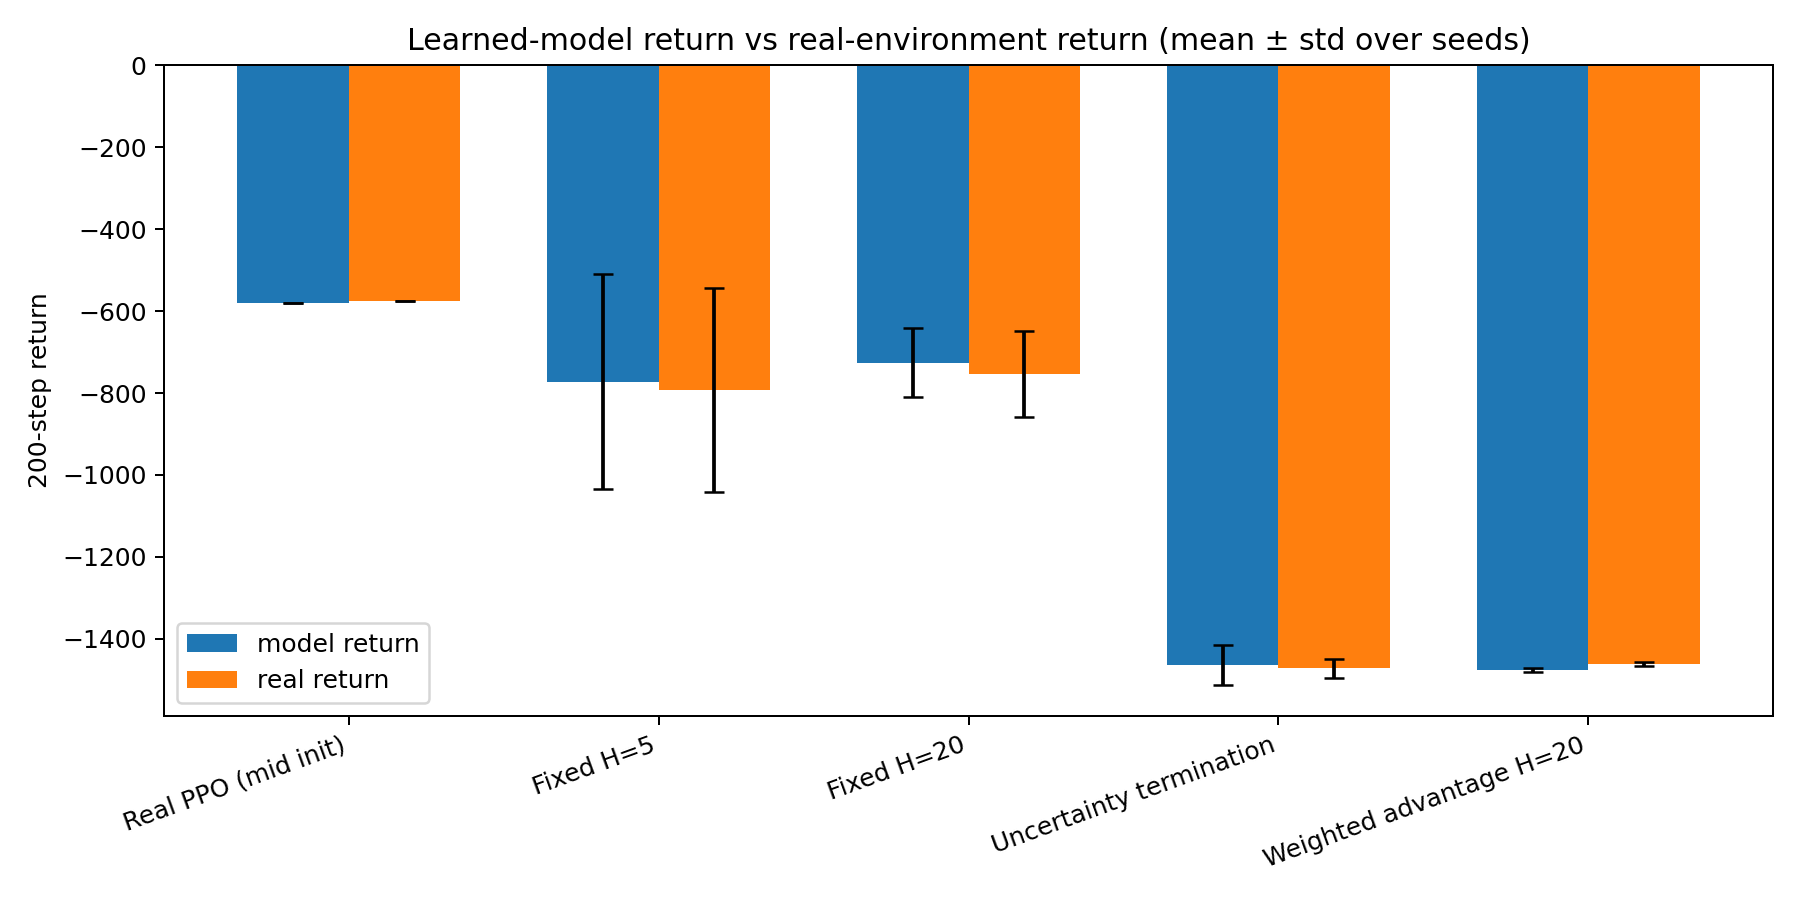
\includegraphics[width=\linewidth]{images/model_vs_real_return_seeds.png}
\caption{Model and environment returns. Error bars for refinement methods show variation across seed means. The shared starting policy has a single checkpoint. The environment is the original Gymnasium simulator.}
\label{fig:returns}
\end{figure}

The stronger-policy comparison starts from the checkpoint that generated the dynamics data and uses approximately 100,000 imagined transitions. It contains one refinement run per method. The starting environment return is $-150.47$. Fixed $H=20$ and uncertainty termination retain returns of $-149.74$ and $-149.83$. Fixed $H=5$ and weighted advantages reach $-295.68$ and $-288.62$. Table~\ref{tab:strong-policy} in the appendix gives the complete recorded comparison.

The existing runs measure the combined effect of the implemented rollout, reward, critic, and optimizer choices. The analytical examples isolate boundary and weighting effects.

\section{Design implications}
\label{sec:discussion}

The analysis points to three concrete questions for world-model policy learning.

\paragraph{What value does the rollout boundary receive?}
An artificial boundary replaces the remaining return with its assigned value. In a task with nonpositive rewards, zero continuation adds the expected omitted cost to the stopped objective. Equation~\eqref{eq:boundary-error} identifies the exact quantity to approximate or constrain. Equation~\eqref{eq:boundary-compensation} gives a separate consistency test: a harmless change of reward origin should receive the corresponding boundary transformation.

\paragraph{Which gradient components does the weight suppress?}
Weighting interacts with the policy parameterization. A weight can turn an advantage component with zero original gradient into a nonzero update. It can also alter the geometry within the representable score space. The finite-action criterion in Section~\ref{sec:weighting} separates these effects. A positive lower bound on weights controls their magnitude; the alignment conditions determine their directional effect.

\paragraph{Which performance quantity is improving?}
Prediction error, model return, return gap, and environment return answer different questions. The Pendulum results illustrate this distinction with matched starts and a common evaluation horizon. A small signed gap can accompany poor control in both systems. Equation~\eqref{eq:return-accounting} keeps environment improvement connected to changes in both model return and optimism.

The existing experiments cover one state-space control task, a fixed learned model, and the recorded policy initializations. The mathematical results cover their stated classes of stopped objectives and local policy updates. Further work can study how these conditions interact with model retraining, shared parameters across decision contexts, and estimated curvature. Those extensions have clear objects to analyze: the boundary approximation error, the score-space residual created by weighting, and the metric used for the update.

\section{Conclusion}

Uncertainty controls enter policy learning through objective choices. Stopping selects a boundary value, and advantage weighting changes the score contributions that form an update. The analysis gives an exact stopping-error formula, a reward-shift criterion, and necessary and sufficient finite-action conditions for universal gradient alignment. Analytical examples expose the consequences when those conditions fail. The continuous-control study gives these questions a concrete implementation and evaluation setting. Together, the results provide a direct way to reason about which parts of imagined learning preserve the intended control objective.

\begin{thebibliography}{99}

\bibitem{pardo}
F. Pardo, A. Tavakoli, V. Levdik, and P. Kormushev.
\newblock Time Limits in Reinforcement Learning.
\newblock \emph{ICML}, PMLR 80:4045--4054, 2018.
\newblock \paperlink{https://proceedings.mlr.press/v80/pardo18a.html}.

\bibitem{tucker}
G. Tucker, S. Bhupatiraju, S. Gu, R. Turner, Z. Ghahramani, and S. Levine.
\newblock The Mirage of Action-Dependent Baselines in Reinforcement Learning.
\newblock \emph{ICML}, PMLR 80:5015--5024, 2018.
\newblock \paperlink{https://proceedings.mlr.press/v80/tucker18a.html}.

\bibitem{mbpo}
M. Janner, J. Fu, M. Zhang, and S. Levine.
\newblock When to Trust Your Model: Model-Based Policy Optimization.
\newblock \emph{NeurIPS}, 2019.
\newblock \paperlink{https://arxiv.org/abs/1906.08253}.

\bibitem{morel}
R. Kidambi, A. Rajeswaran, P. Netrapalli, and T. Joachims.
\newblock MOReL: Model-Based Offline Reinforcement Learning.
\newblock \emph{NeurIPS}, 2020.
\newblock \paperlink{https://arxiv.org/abs/2005.05951}.

\bibitem{mopo}
T. Yu, G. Thomas, L. Yu, S. Ermon, J. Zou, S. Levine, C. Finn, and T. Ma.
\newblock MOPO: Model-based Offline Policy Optimization.
\newblock \emph{NeurIPS}, 2020.
\newblock \paperlink{https://arxiv.org/abs/2005.13239}.

\bibitem{tatu}
J. Zhang, J. Lyu, X. Ma, J. Yan, J. Yang, L. Wan, and X. Li.
\newblock Uncertainty-Driven Trajectory Truncation for Data Augmentation in Offline Reinforcement Learning.
\newblock \emph{ECAI}, 2023.
\newblock \paperlink{https://arxiv.org/abs/2304.04660}.

\bibitem{ppo}
J. Schulman, F. Wolski, P. Dhariwal, A. Radford, and O. Klimov.
\newblock Proximal Policy Optimization Algorithms.
\newblock arXiv:1707.06347, 2017.
\newblock \paperlink{https://arxiv.org/abs/1707.06347}.

\bibitem{gae}
J. Schulman, P. Moritz, S. Levine, M. I. Jordan, and P. Abbeel.
\newblock High-Dimensional Continuous Control Using Generalized Advantage Estimation.
\newblock \emph{ICLR}, 2016.
\newblock \paperlink{https://arxiv.org/abs/1506.02438}.

\bibitem{pets}
K. Chua, R. Calandra, R. McAllister, and S. Levine.
\newblock Deep Reinforcement Learning in a Handful of Trials using Probabilistic Dynamics Models.
\newblock \emph{NeurIPS}, 2018.
\newblock \paperlink{https://arxiv.org/abs/1805.12114}.

\bibitem{sutton}
R. S. Sutton, D. A. McAllester, S. P. Singh, and Y. Mansour.
\newblock Policy Gradient Methods for Reinforcement Learning with Function Approximation.
\newblock \emph{Advances in Neural Information Processing Systems}, 12, 1999.
\newblock \paperlink{https://papers.nips.cc/paper_files/paper/1999/hash/464d828b85b0bed98e80ade0a5c43b0f-Abstract.html}.

\bibitem{kakade}
S. M. Kakade.
\newblock A Natural Policy Gradient.
\newblock \emph{Advances in Neural Information Processing Systems}, 14, 2001.
\newblock \paperlink{https://proceedings.neurips.cc/paper_files/paper/2001/hash/4b86abe48d358ecf194c56c69108433e-Abstract.html}.

\bibitem{agarwal}
A. Agarwal, S. M. Kakade, J. D. Lee, and G. Mahajan.
\newblock On the Theory of Policy Gradient Methods: Optimality, Approximation, and Distribution Shift.
\newblock \emph{Journal of Machine Learning Research}, 22(98):1--76, 2021.
\newblock \paperlink{https://www.jmlr.org/papers/v22/19-736.html}.

\bibitem{awr}
X. B. Peng, A. Kumar, G. Zhang, and S. Levine.
\newblock Advantage-Weighted Regression: Simple and Scalable Off-Policy Reinforcement Learning.
\newblock arXiv:1910.00177, 2019.
\newblock \paperlink{https://arxiv.org/abs/1910.00177}.

\bibitem{osband}
I. Osband.
\newblock Delightful Policy Gradient.
\newblock arXiv:2603.14608v1, 2026.
\newblock \paperlink{https://arxiv.org/abs/2603.14608v1}.

\bibitem{han}
S. Han and Z. Hu.
\newblock Baselines and Score Centering in Policy Gradient Estimation.
\newblock arXiv:2610.22263v1, 2026.
\newblock \paperlink{https://arxiv.org/abs/2610.22263v1}.

\bibitem{world4rl}
Z. Jiang, K. Liu, Y. Qin, S. Tian, Y. Zheng, M. Zhou, C. Yu, H. Li, and D. Zhao.
\newblock World4RL: Diffusion World Models for Policy Refinement with Reinforcement Learning for Robotic Manipulation.
\newblock arXiv:2509.19080v1, 2025.
\newblock \paperlink{https://arxiv.org/abs/2509.19080v1}.

\bibitem{wovr}
Z. Jiang, S. Zhou, Y. Jiang, Z. Huang, M. Wei, Y. Chen, T. Zhou, Z. Guo, H. Lin, Q. Zhang, Y. Wang, H. Li, C. Yu, and D. Zhao.
\newblock WoVR: World Models as Reliable Simulators for Post-Training VLA Policies with RL.
\newblock arXiv:2602.13977v1, 2026.
\newblock \paperlink{https://arxiv.org/abs/2602.13977v1}.

\end{thebibliography}

\appendix
\section{A bounded-reward Gaussian construction}
\label{app:gaussian}

The finite-action analysis isolates the role of the score space. The following construction shows that positive weighting can also reverse the mean update of a scalar Gaussian actor.

\begin{proposition}[Direction reversal for a continuous actor]
\label{prop:gaussian}
Let $Z\sim\mathcal N(\theta,1)$ and let
\[
r(Z)=\sin Z-\sin(2Z)-2,\qquad
w(Z)=\frac1{50}+\frac{49}{50}e^{-Z^2}.
\]
At $\theta=0$, use the exact advantage and hold $w$ fixed in the surrogate derivative. Then the expected-return gradient is positive and the weighted score gradient is negative. The conclusion also holds for the bounded action $a=2\tanh Z$, with the reward and weight expressed through $Z=\operatorname{atanh}(a/2)$. If the actor also learns its log standard deviation $\eta$, the full two-parameter gradient reverses at $(\theta,\eta)=(0,0)$.
\end{proposition}

\begin{proof}
The reward lies in $[-4,0]$. Symmetry gives $\E r=-2$ at $\theta=0$, so the exact advantage is $A(Z)=\sin Z-\sin(2Z)$. The score for the Gaussian mean is $Z$ there. Differentiating its characteristic function gives
\[
\E[Z\sin(kZ)]=ke^{-k^2/2}.
\]
The derivative is justified by $\E|Z|<\infty$. Completing the square in the Gaussian integral gives
\[
\E[e^{-Z^2}Z\sin(kZ)]
=\frac{k}{3\sqrt3}e^{-k^2/6}.
\]
Consequently,
\begin{align}
g&=e^{-1/2}-2e^{-2}>0,\\
g_w&=\frac1{50}g+
\frac{49}{150\sqrt3}\left(e^{-1/6}-2e^{-2/3}\right).
\label{eq:gaussian-gradient}
\end{align}
The first sign uses $e^{3/2}>2$. To check the second sign with explicit bounds, the alternating Taylor bounds for $e^{-x}$ on $0<x<1$ give
\[
2e^{-2/3}-e^{-1/6}
\ge 2\left(1-\frac23+\frac29-\frac4{81}\right)
-\left(1-\frac16+\frac1{72}\right)
=\frac{107}{648}.
\]
Since $g<1$ and $\sqrt3<2$,
\[
g_w<\frac1{50}-\frac{49}{300}\frac{107}{648}<0.
\]
For differentiating the expected reward in $\theta$, the reward is bounded and the Gaussian density derivative on a bounded neighborhood of zero has an integrable Gaussian envelope times a linear factor. Dominated convergence therefore identifies $g$ with the derivative of the expected return.

For the family $Z\sim\mathcal N(\theta,e^{2\eta})$, the log-scale score at $(0,0)$ is $Z^2-1$. Differentiation in $\eta$ is justified by a Gaussian envelope times a quadratic factor. The advantage is odd, and the weight and log-scale score are even. Both the unweighted and weighted log-scale gradients therefore vanish. The full gradients are $(g,0)^\top$ and $(g_w,0)^\top$, whose inner product is negative.

Under $a=2\tanh Z$, the density Jacobian at a fixed action is independent of both parameters, so the scores are unchanged. The same expectations and signs apply. Values assigned to the reward at $a=\pm2$ have probability zero and can be chosen in $[-4,0]$.
\end{proof}

The weight satisfies $0.02<w\le1$ and can be written in the form of \eqref{eq:implemented-weight}: choose $u(z)=-(\tau_u/\beta)\log w(z)$ with $\beta,\tau_u>0$. This represents an admissible fixed confidence signal. The construction analyzes the weighting operation; the signal is specified analytically.

\section{The local PPO derivative and advantage centering}
\label{app:ppo}

Let $\theta_0$ be the reference policy, and hold sampled advantages and weights fixed. For a finite action space, define the exact expected clipped surrogate
\[
L_w(\theta)=\E_{p}\min\left\{\rho_\theta wA,\operatorname{clip}(\rho_\theta,1-\epsilon,1+\epsilon)wA\right\}.
\]
Here $\rho_\theta=\pi_\theta/\pi_{\theta_0}$ and $\epsilon>0$.

At $\theta=\theta_0$, every ratio equals one. Full support and differentiability give a neighborhood in which all finitely many ratios lie inside the clipping interval. Thus
\begin{equation}
\nabla L_w(\theta_0)=\E_p[wA\psi]=g_w(A).
\end{equation}
This equality concerns the initial expected surrogate derivative. A positive common rescaling of exact centered advantages preserves its direction.

Extending the weighted score sum to all advantage vectors, for an arbitrary centering constant $c$,
\begin{equation}
g_w(A-c)=g_w(A)-c\E_p[w\psi].
\label{eq:weighted-baseline}
\end{equation}
Action-dependent weights can therefore make the choice of center affect the update. Related baseline and score-centering effects are analyzed in \cite{tucker,han}. In the experiments, centering and scaling use each minibatch, the critic provides GAE estimates, and PPO performs several Adam updates. The exact local analysis identifies the expected weighting operation before those additional choices.

\section{The stronger-policy comparison}
\label{app:strong-policy}

\begin{table}[htbp]
\centering
\small
\caption{Refinement from the stronger policy, with one run per method. Values are means $\pm$ sample standard deviations across 50 matched evaluation episodes. Each episode has 200 steps. These spreads describe episodes within a checkpoint.}
\label{tab:strong-policy}
\begin{tabular}{lrrr}
\toprule
Method & Environment return & Return gap & Final length\\
\midrule
Starting policy & $-150.47\pm86.30$ & $-0.12\pm0.55$ & ---\\
Fixed $H=5$ & $-295.68\pm294.85$ & $2.03\pm8.19$ & $5.00$\\
Fixed $H=20$ & $-149.74\pm86.59$ & $-0.19\pm0.40$ & $20.00$\\
Uncertainty termination & $-149.83\pm86.96$ & $-0.20\pm0.48$ & $16.40$\\
Weighted advantage & $-288.62\pm282.46$ & $9.75\pm25.40$ & $20.00$\\
\bottomrule
\end{tabular}
\end{table}

\begin{figure}[htbp]
\centering
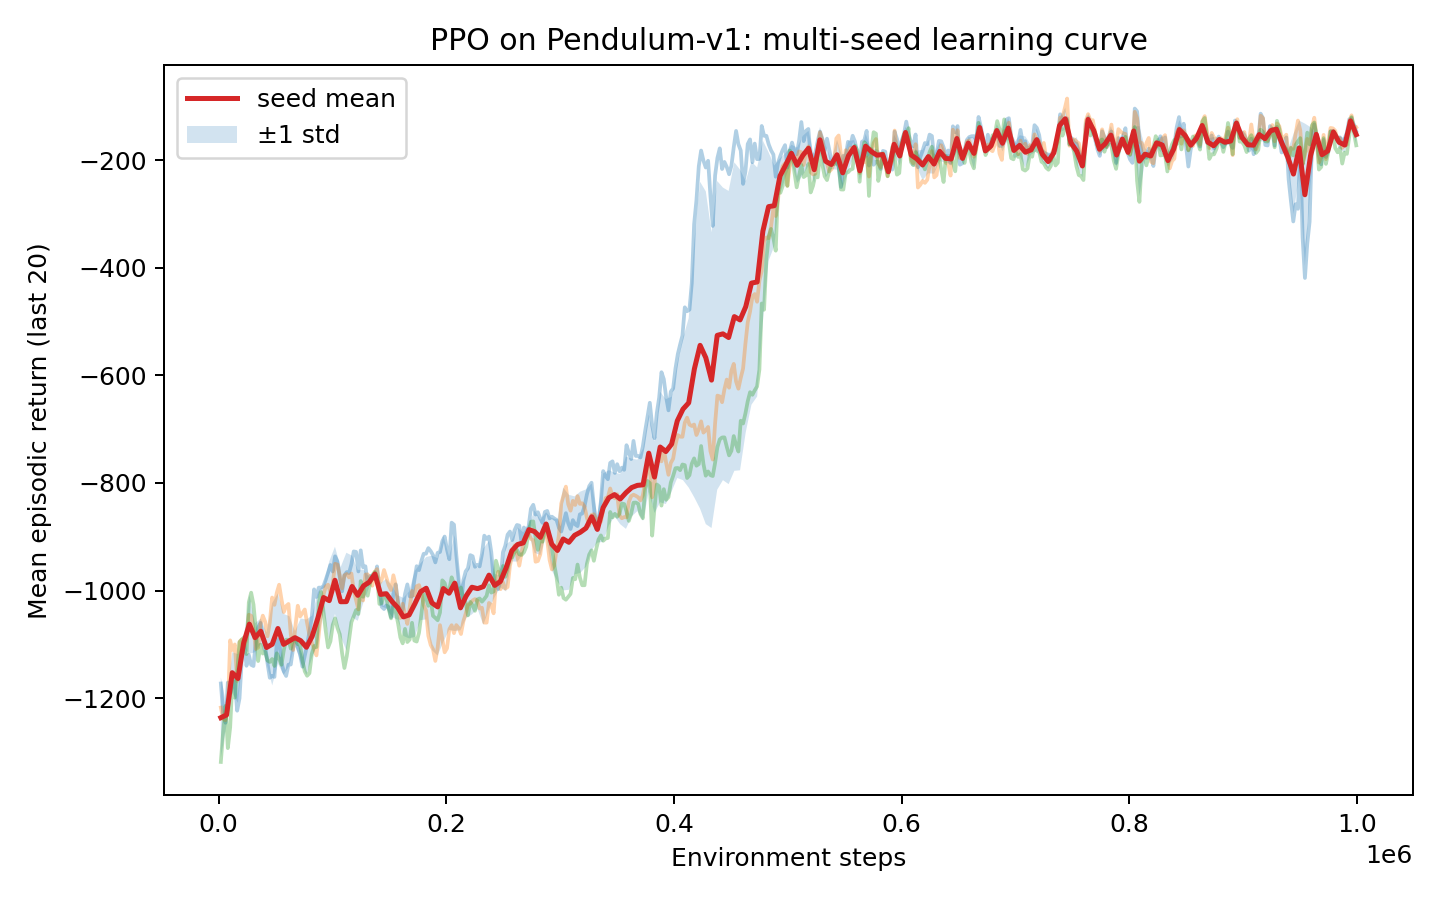
\includegraphics[width=0.84\linewidth]{images/learning_curve_mean_std.png}
\caption{Training curves for the three original PPO seeds. The deterministic evaluation means are $-148.7$, $-152.7$, and $-157.5$.}
\label{fig:ppo}
\end{figure}

\section{Code and result sources}

The repository at \url{https://github.com/TanhJK728/reliable-world-model-rl} contains the implementation and the recorded result tables. The analysis maps to the following components:

\begin{center}
\small
\begin{tabular}{p{0.39\linewidth}p{0.55\linewidth}}
\toprule
Component & Role in this paper\\
\midrule
\code{imagined\_env.py} & Segment stopping, exact reward, successor state, and reset rule.\\
\code{train\_imagined\_ppo.py} & Boundary masking in GAE and positive weights applied after advantage centering.\\
\code{ppo\_core.py} & Gaussian actor, action-density transformation, and reward function.\\
\code{world\_model.py} & Memberwise state projection, averaging, and disagreement.\\
\code{compare\_imagined\_methods.py} & Model and environment evaluation from matched starts.\\
\code{aggregate\_comparison.py} & Stored summaries across refinement seeds.\\
\bottomrule
\end{tabular}
\end{center}

\begingroup\raggedright\small
Table~\ref{tab:refinement} uses the recorded summary in \path{runs/comparison_seeds/comparison_aggregated.csv}. Table~\ref{tab:strong-policy} uses \path{runs/comparison/comparison.csv}. Prediction measurements come from \path{runs/world_model_eval/one_step_results.csv} and \path{runs/world_model_eval/rollout_results.csv}. PPO evaluation comes from \path{runs/ppo_summary/evaluation.csv}. These records provide the numerical sources for the tables and figures in this paper.
\par\endgroup

\end{document}
